\documentclass[aspectratio=169]{beamer}

\usepackage[T1]{fontenc}
\usepackage{amsmath}
\usepackage{amssymb}
\usepackage{graphicx}
\usepackage{tikz}
\usetikzlibrary{shapes.geometric, arrows.meta, positioning}

\definecolor{coolpurple}{HTML}{7f65a0}
\definecolor{lightpurple}{HTML}{ede8f5}
\definecolor{darktext}{HTML}{1a1a2e}
\definecolor{highlightpurple}{HTML}{5a3e82}

\setbeamercolor{normal text}{fg=darktext, bg=white}
\setbeamercolor{structure}{fg=coolpurple}
\setbeamercolor{frametitle}{fg=white, bg=coolpurple}
\setbeamercolor{title}{fg=white, bg=coolpurple}
\setbeamercolor{subtitle}{fg=white}
\setbeamercolor{date}{fg=coolpurple}
\setbeamercolor{author}{fg=coolpurple}
\setbeamercolor{item}{fg=coolpurple}
\setbeamercolor{subitem}{fg=coolpurple!70!black}
\setbeamercolor{block title}{bg=coolpurple, fg=white}
\setbeamercolor{block body}{bg=lightpurple, fg=darktext}
\setbeamercolor{alerted text}{fg=highlightpurple}

\setbeamertemplate{itemize item}{\color{coolpurple}$\blacktriangleright$}
\setbeamertemplate{itemize subitem}{\color{coolpurple!70}$\bullet$}
\setbeamertemplate{navigation symbols}{}
\setbeamertemplate{footline}{%
	\hfill\insertframenumber\,/\,\inserttotalframenumber\hspace{1em}\vspace{0.5em}
}

\newcommand{\hl}[1]{\textcolor{coolpurple}{\textbf{#1}}}
\newcommand{\R}{\mathbb{R}}

\title{EngageNet}
\subtitle{M3 Presentation - May 31, 2026}
\author{Lado Turmanidze, Luka Javakhishvili, Mariami Gadelia, Keso Chikhladze}
\institute{\small{Supervisors: Dr. Philipp M\"{u}ller \& Beso Mikaberidze}}
\date{May 31, 2026}

\begin{document}

	\begin{frame}
		\titlepage
	\end{frame}

	\begin{frame}{Today's Agenda}
		\begin{enumerate}
			\item \textbf{Full architecture recap} - end-to-end data flow
			\item \textbf{Beta distribution justification} - why not Kumaraswamy or logit-normal?
			\item \textbf{Implementation} - JAX + Flax Linen, project structure
			\item \textbf{Engineering beyond the paper} - what research papers never show
			\item \textbf{Evaluation metrics} - CCC and CDD
			\item \textbf{Status \& next steps}
		\end{enumerate}
	\end{frame}


	\begin{frame}{\textsc{Part 1:} Full Architecture - Data Flow}
		\centering
		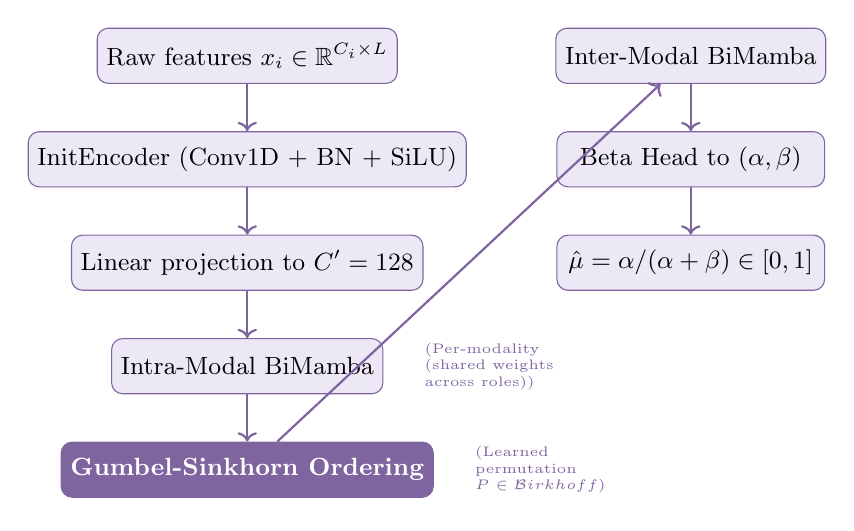
\begin{tikzpicture}[
			node distance=0.6cm, 
			font=\small,
			box/.style={draw=coolpurple, fill=lightpurple, rounded corners,
				minimum width=3.4cm, minimum height=0.7cm, align=center}
			]

			\node[box] (input) {Raw features $x_i \in \mathbb{R}^{C_i \times L}$};
			\node[box, below=of input] (enc) {InitEncoder (Conv1D + BN + SiLU)};
			\node[box, below=of enc] (proj) {Linear projection to $C'=128$};
			\node[box, below=of proj] (intra) {Intra-Modal BiMamba};
			\node[box, below=of intra, fill=coolpurple, text=white, font=\small\bfseries] (gs) {Gumbel-Sinkhorn Ordering};
			
			\node[box, right=2.0cm of input] (inter) {Inter-Modal BiMamba};
			\node[box, below=of inter] (beta) {Beta Head to $(\alpha, \beta)$};
			\node[box, below=of beta] (out) {$\hat{\mu} = \alpha / (\alpha + \beta) \in [0,1]$};
	
			\foreach \a/\b in {input/enc, enc/proj, proj/intra, intra/gs, gs/inter, inter/beta, beta/out} {
				\draw[->, thick, coolpurple] (\a) -- (\b);
			}
			
			\node[right=0.4cm of intra, text=coolpurple, font=\tiny, align=left] 
			{(Per-modality \\ (shared weights \\ across roles))};
			
			\node[right=0.4cm of gs, text=coolpurple, font=\tiny, align=left] 
			{(Learned \\ permutation \\ $P \in \mathcal{B}irkhoff$)};
			
		\end{tikzpicture}
	\end{frame}

	\begin{frame}{Architecture - Key Design Choices}
		\begin{columns}[onlytextwidth]
			\begin{column}{0.48\textwidth}
				\begin{block}{Selective State Space (SSM)}
					\small
					\begin{itemize}
						\item Input-dependent $\Delta_t, B_t, C_t$
						\item $O(\log L)$ via associative scan
						\item Bidirectional: forward + reversed
					\end{itemize}
				\end{block}
				\begin{block}{Weight Sharing}
					\small
					Same encoder for expert \& novice of the same modality $\to$ 10 encoders, not 20.
				\end{block}
			\end{column}
			\begin{column}{0.48\textwidth}
				\begin{block}{Inter-Modal Fusion}
					\small
					\begin{itemize}
						\item Transpose: time $\leftrightarrow$ modality
						\item BiMamba across $\sum C_i'$ axis
						\item Order learned via Gumbel-Sinkhorn
					\end{itemize}
				\end{block}
				\begin{block}{Core Modalities (4)}
					\small
					FAUs, gaze, pose, audio (eGeMAPS). Chosen for temporal richness \& complementarity.
				\end{block}
			\end{column}
		\end{columns}
	\end{frame}


	\begin{frame}{\textsc{Part 2:} Why Beta? - Comparison with Alternatives}
		\begin{columns}[onlytextwidth]
			\begin{column}{0.48\textwidth}
				\begin{block}{Requirements}
					\small
					\begin{enumerate}
						\item Support on $[0,1]$ (no leakage)
						\item Closed-form variance at inference
						\item Closed-form KL for TTA loss
						\item Differentiable for backprop
					\end{enumerate}
				\end{block}
			\end{column}
			\begin{column}{0.48\textwidth}
				\begin{block}{Scorecard}
					\footnotesize
					\begin{tabular}{lccc}
						& Beta & Kuma. & Logit-N \\
						\hline
						Support $[0,1]$ & \checkmark & \checkmark & \checkmark \\
						Var (closed) & \checkmark & $\times$ & $\times$ \\
						KL (closed) & \checkmark & $\times$ & $\sim$ \\
						Fast inference & \checkmark & $\times$ & $\times$ \\
					\end{tabular}
				\end{block}
			\end{column}
		\end{columns}
	\end{frame}

	\begin{frame}{Beta vs Kumaraswamy - The Inference Cost}
		\begin{columns}[onlytextwidth]
			\begin{column}{0.50\textwidth}
				\begin{alertblock}{Kumaraswamy variance}
					\small
					Requires $\Gamma$ function evaluations:
					$$ \text{Var}[Y] = b\,B\!\left(1{+}\tfrac{2}{a},b\right) - \left[b\,B\!\left(1{+}\tfrac{1}{a},b\right)\right]^2 $$
					Expensive at 25 Hz real-time streaming.
				\end{alertblock}
			\end{column}
			\begin{column}{0.46\textwidth}
				\begin{block}{Beta variance}
					\small
					Pure arithmetic:
					$$ U(x) = \frac{\alpha\beta}{(\alpha{+}\beta)^2(\alpha{+}\beta{+}1)} $$
					\hl{No transcendental functions at inference.}
				\end{block}
			\end{column}
		\end{columns}
		\vspace{0.5em}
		\centering\small
		Monotonic proxy: $\partial U/\partial\kappa < 0$ and $\partial H/\partial\kappa < 0$ $\implies$ variance ranks samples identically to differential entropy.
	\end{frame}

	\begin{frame}{Beta vs Logit-Normal - The KL Problem}
		\begin{columns}[onlytextwidth]
			\begin{column}{0.50\textwidth}
				\begin{alertblock}{Logit-Normal issues}
					\small
					\begin{itemize}
						\item Moments need numerical integration
						\item KL in $[0,1]$ space: no closed form
						\item Gradients explode near boundaries
					\end{itemize}
				\end{alertblock}
			\end{column}
			\begin{column}{0.46\textwidth}
				\begin{block}{Beta KL (closed-form)}
					\footnotesize
					\resizebox{\textwidth}{!}{%
						$D_{KL}(B_1\|B_2) = \ln\tfrac{B_2}{B_1} + (\alpha_1{-}\alpha_2)\psi(\alpha_1) + \cdots$
					}
					\vspace{0.3em}

					\small Exact, stable, used directly in $\mathcal{L}_{\text{mis}}$ for TTA.
				\end{block}
			\end{column}
		\end{columns}
		\vspace{0.6em}
		\begin{center}
			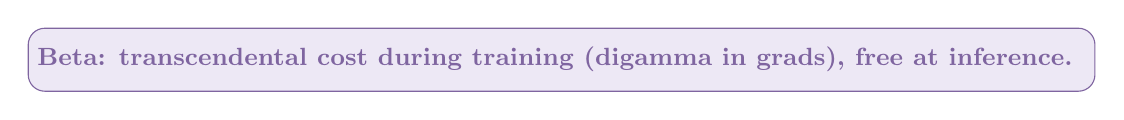
\begin{tikzpicture}
				\node[draw=coolpurple, fill=lightpurple, rounded corners=6pt,
				minimum width=10cm, minimum height=0.8cm, align=center,
				font=\small\bfseries, text=coolpurple] {
					Beta: transcendental cost during training (digamma in grads), free at inference.
				};
			\end{tikzpicture}
		\end{center}
	\end{frame}

	\begin{frame}{\textsc{Part 3:} Implementation - JAX + Flax Linen}
		\begin{columns}[onlytextwidth]
			\begin{column}{0.48\textwidth}
				\begin{block}{Why JAX?}
					\small
					\begin{itemize}
						\item \texttt{jax.lax.associative\_scan} for $O(\log L)$ SSM
						\item XLA compilation
						\item Functional transforms: \texttt{jit}, \texttt{grad}
						\item I wanted to see what the hype was about
					\end{itemize}
				\end{block}
			\end{column}
			\begin{column}{0.48\textwidth}
				\begin{block}{Why Flax Linen?}
					\small
					\begin{itemize}
						\item \texttt{nn.Module} with explicit params
						\item Kinda like functional programming (I love OCaml)
						\item Seamless Orbax checkpointing
						\item Clean separation: model vs state
					\end{itemize}
				\end{block}
			\end{column}
		\end{columns}
		\vspace{0.5em}
		\centering\small
		All randomness controlled via \texttt{jax.random.PRNGKey(95)} with explicit key splitting.
	\end{frame}

	\begin{frame}{Project Structure}
		\begin{columns}[onlytextwidth]
			\begin{column}{0.46\textwidth}
				\begin{block}{\texttt{src/} - Core modules}
					\footnotesize
					\begin{tabular}{ll}
						\texttt{config.py} & Centralised cnfg \\
						\texttt{ssm.py} & JAX assoc. scan \\
						\texttt{bimamba.py} & BiMambaBlock \\
						\texttt{inter\_modal.py} & Gumbel-Sinkhorn \\
						\texttt{beta\_head.py} & Beta regression \\
						\texttt{model.py} & Full EngageNet \\
						\texttt{init\_encoder.py} & Shallow CNN \\
						\texttt{modality\_frontend.py} & Per-modality entry \\
					\end{tabular}
				\end{block}
			\end{column}
			\begin{column}{0.50\textwidth}
				\begin{block}{\texttt{src/} - Pipeline \& eval}
					\footnotesize
					\begin{tabular}{ll}
						\texttt{train.py} & AdamW + early stop \\
						\texttt{tta.py} & Test-time adaptation \\
						\texttt{inference.py} & Multi-corpus CSV out \\
						\texttt{dataset.py} & Lazy streaming loader \\
						\texttt{data\_loader.py} & Batch iterator \\
						\texttt{metrics.py} & CCC, CDD \\
						\texttt{evaluate.py} & Scoring script \\
						\texttt{aggregator.py} & Overlap-add windows \\
					\end{tabular}
				\end{block}
			\end{column}
		\end{columns}
	\end{frame}

	\begin{frame}{\textsc{Part 4:} What We Added Beyond the Paper}
		\begin{columns}[onlytextwidth]
			\begin{column}{0.48\textwidth}
				\begin{block}{Data engineering?}
					\small
					\begin{itemize}
						\item Lazy streaming for 88+ GiB dataset (one session at a time in memory)
						\item Dynamic \texttt{active\_modalities} filter
					\end{itemize}
				\end{block}
				\begin{block}{Reproducibility}
					\small
					\begin{itemize}
						\item CLI via \texttt{EngageNetConfig.from\_cli()}
						\item Orbax checkpoints every $N$ epochs
						\item Docker containers (train + inference)
					\end{itemize}
				\end{block}
			\end{column}
			\begin{column}{0.48\textwidth}
				\begin{block}{Training details}
					\small
					\begin{itemize}
						\item Tau annealing: $\tau_t = \max(\tau_\infty, \tau_0 \cdot \gamma^t)$
						\item CCC-based validation + early stopping
						\item AdamW with weight decay
					\end{itemize}
				\end{block}
				\begin{block}{Inference pipeline}
					\small
					\begin{itemize}
						\item Per-session processing
						\item Overlap-add window aggregation
						\item Submission CSV generation
					\end{itemize}
				\end{block}
			\end{column}
		\end{columns}
	\end{frame}

	\begin{frame}{Surgical TTA - Implementation Choices}
		\begin{columns}[onlytextwidth]
			\begin{column}{0.48\textwidth}
				\begin{block}{Frozen vs updated}
					\small
					\begin{itemize}
						\item \hl{Updated:} BatchNorm, first Conv1D in InitEncoder, first Dense in inter-modal
						\item \hl{Frozen:} All SSM params, Beta head, intra-modal BiMamba weights
					\end{itemize}
				\end{block}
			\end{column}
			\begin{column}{0.48\textwidth}
				\begin{block}{Why surgical?}
					\small
					\begin{itemize}
						\item Prevents catastrophic forgetting
						\item Mitigates Variance Starvation: model cannot inflate $\text{Var}[y]$ to bypass hard samples
						\item Only 3--5\% of total params updated
					\end{itemize}
				\end{block}
			\end{column}
		\end{columns}
	\end{frame}

	%% PART 5: EVALUATION
	\begin{frame}{\textsc{Part 5:} Evaluation Metrics}
		\begin{columns}[onlytextwidth]
			\begin{column}{0.50\textwidth}
				\begin{block}{CCC (primary metric)}
					\small
					$$ \text{CCC} = \frac{2\rho\,\sigma_{\hat{y}}\sigma_y}{\sigma_{\hat{y}}^2 + \sigma_y^2 + (\mu_{\hat{y}}-\mu_y)^2} $$
					Penalises both scale and location shift. Combined: $\frac{1}{N}\sum_n \text{CCC}_n$.
				\end{block}
			\end{column}
			\begin{column}{0.46\textwidth}
				\begin{block}{CDD (fairness)}
					\small
					$$ \text{CDD} = \frac{1}{|G|}\sum_{g} |\text{CCC}_g - \text{CCC}_{\text{all}}| $$
					Computed per gender and per language. Lower = more equitable.
				\end{block}
			\end{column}
		\end{columns}
		\vspace{0.6em}
		\centering\small
		Challenge ranking: maximise CCC while keeping CDD below threshold.
	\end{frame}

	%% PART 6: STATUS
	\begin{frame}{Status \& Next Steps}
		\begin{columns}[onlytextwidth]
			\begin{column}{0.48\textwidth}
				\begin{block}{Done \checkmark}
					\small
					\begin{itemize}
						\item Full architecture coded
						\item All unit tests pass
						\item Docker containers ready
						\item Paper draft in solid shape
					\end{itemize}
				\end{block}
			\end{column}
			\begin{column}{0.48\textwidth}
				\begin{block}{In Progress \& Next Steps}
					\small
					\begin{itemize}
						\item Using MICM compute for training
						\item Training on NoXi
						\item Hyperparameter tuning?
						\item TTA evaluation on NoXi+J
					\end{itemize}
				\end{block}
			\end{column}
		\end{columns}
		\vspace{0.8em}
		\begin{center}
			\Large\bfseries\color{coolpurple} Questions?
		\end{center}
	\end{frame}

\end{document}

